%!TEX root = ../report.tex
\chapter{Architectural business information}
\label{ch:business}
The following section describes the different aspects of the business environment of the Smart Flood Monitor. First we will explain our vision and why there is place for us at the market. After this the product and its customers will be explained. This chapter is completed with a more detailed look at the business model and some models about the market and the financial prospect.

\section{Business opportunity}
There are many natural disasters happening each year all over the world. Each year these disasters take lives, waste a lot of property and money and cause social disturbance. It is expected that natural disasters will cause \$300 billion in losses annually in the upcoming decade. Climate change causes the natural disasters to get worse every year. Also the number of natural disasters has increased significantly since 1970.\\
Looking at, for example, the Indian ocean's tsunami in 2004, it looks that the damage could have been significantly reduced if the necessary people were warned. A system that would reduce the damage of natural disaster, could result in billions. \\
A system that warns and guides the people before or during the floods can result in billions being saved and will save allot of lives.

\section{Vision statement}
The Smart Flood Monitor will cause a revolutionary innovation on the environmental monitoring market. \CompanyName will offer a system which can detect floods early and correctly. This system helps us to enforce our vision, to limit the social and financial consequences of floods and avoid the loss of human lives. 

\CompanyName will not be the only competitor on the environmental monitoring market. This means \CompanyName will have to take their own strength and weaknesses into account. If we combine these qualities with an analysis of the opportunities and weaknesses on the market, we should be able to become a core part of the future environmental monitoring systems.\\\\

Such an analysis is called a SWOT-analysis. 

%%Strengths
%\newcommand{\Strengths}{
%An easily adjustable system that is future proof \\
%Having a low selling place. Lower then the compatitors \\
%Having a good management team \\
%Frequent discussion with technical and business experts in the field. \\
%Main features don't focus on user-interaction. \\
%Having a reletively big project team \\
%Financial stability \\
%}
%
%\newcommand{\Weaknesses}{
%Decisions need to be made by the entire project team. There is a higher chance of a difference of opinion is members, holding back the project and leads to time wastes \\
%No experience with creating such system \\
%Some main features rely on country-specific systems \\
%}
%
%\newcommand{\Opportunities}{
%Due to climate change, the market will grow and such a system becomes more urgent \\
%With a bigger program team, the pros and cons of the decisions are more clear \\
%Allowing the system to be flexible so it can also be used for other kinds of monitoring activities \\
%Adding more ways the system can the people in dangerous areas \\
%Though the team doesn't have direct experience in this field, the team does have experience with specific parts of the system \\
%Allowing the system to support and use the newest sensors in order to obtain more, and a wider variaty of, information \\
%}
%
%\newcommand{\Threats}{
%New competitors will enter the market and Climate change will force to improve the system over time. \\
%Changes of the external systems that our system uses to properly communicate. \\
%The sizes of certain area's to monitor can be too big to get a good and reliable view of them \\
%}

\newcommand{\SwotItems}[1]{
	\begin{itemize}
	%\begin{minipage}[t][8cm]{5cm}
		#1
	%\end{minipage}	
	\end{itemize}
}

%Strengths
\newcommand{\Strengths}{
\SwotItems{
	\item An easily adjustable system that is future proof
	\item Having a low selling price. Lower then the competitors
	\item Having a good management team
	\item Frequent discussion with technical and business experts in the field.
	\item Main features don't focus on user-interaction.
	\item Having a relatively big project team
	\item Financial stability
}
}

\newcommand{\Weaknesses}{
\SwotItems{
	\item Decisions need to be made by the entire project team. There is a higher chance of a difference of opinion is members, holding back the project and leads to time wastes
	\item No experience with creating such system
	\item Some main features rely on country-specific systems
}
}

\newcommand{\Opportunities}{
\SwotItems{
	\item Due to climate change, the market will grow and such a system becomes more urgent
	\item With a bigger program team, the pros and cons of the decisions are more clear
	\item Allowing the system to be flexible so it can also be used for other kinds of monitoring activities
	\item Adding more ways the system can the people in dangerous areas
	\item Though the team doesn't have direct experience in this field, the team does have experience with specific parts of the system
	\item Allowing the system to support and use the newest sensors in order to obtain more, and a wider variaty of, information
}
}

\newcommand{\Threats}{
\SwotItems{
	\item New competitors will enter the market and Climate change will force to improve the system over time.
	\item Changes of the external systems that our system uses to properly communicate.
	\item The sizes of certain area's to monitor can be too big to get a good and reliable view of them
}
}

\usetikzlibrary{matrix}

\colorlet{helpful}{lime!70}
\colorlet{harmful}{red!30}
\colorlet{internal}{yellow!20}
\colorlet{external}{cyan!30}
\colorlet{S}{helpful!50!internal}
\colorlet{W}{harmful!50!internal}
\colorlet{O}{helpful!50!external}
\colorlet{T}{harmful!50!external}

\newcommand{\texta}{Helpful\\ \tiny (to achieve the objective)\par}
\newcommand{\textb}{Harmful\\ \tiny (to achieve the objective)\par}
\newcommand{\textcn}{Internal origin\\ \tiny (product\slash company attributes)\par}
\newcommand{\textdn}{External origin\\ \tiny (environment\slash market attributes)\par}

\newcommand{\back}[1]{\fontsize{60}{70}\selectfont #1}

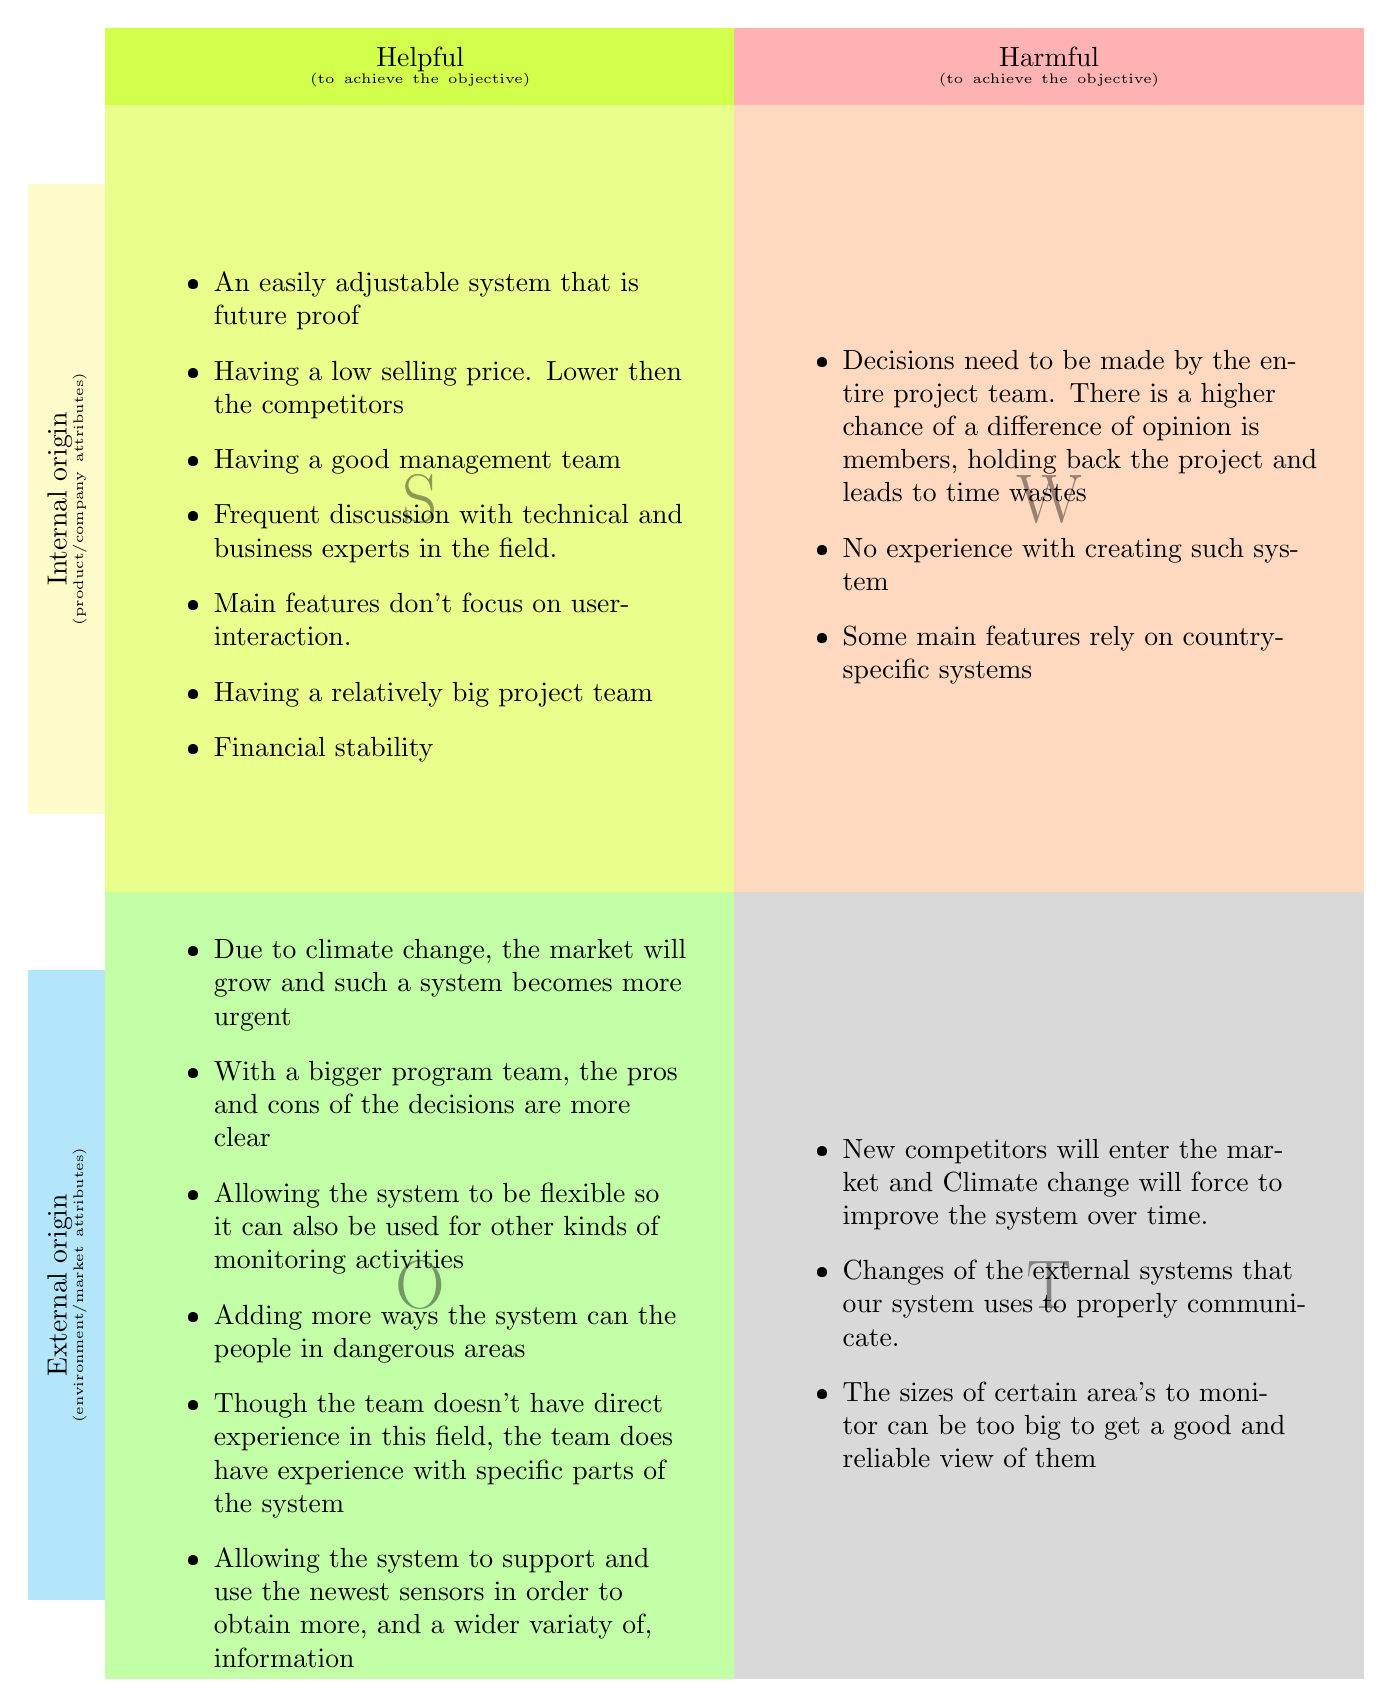
\begin{tikzpicture}[
    any/.style={minimum width=8cm,minimum height=10cm,%
                 text width=7cm,align=center,outer sep=0pt},
    header/.style={any,minimum height=1cm,fill=black!10},
    leftcol/.style={header,rotate=90},
    mycolor/.style={fill=#1, text=#1!60!black}
]

\matrix (SWOT) [matrix of nodes,nodes={any,anchor=center},%
                column sep=-\pgflinewidth,%
                row sep=-\pgflinewidth,%
                row 1/.style={nodes=header},%
                column 1/.style={nodes=leftcol},
                inner sep=0pt]
{
          &|[fill=helpful]| {\texta} & |[fill=harmful]| {\textb} \\
|[fill=internal]| {\textcn} & |[mycolor=S]| \back{S} & |[mycolor=W]| \back{W} \\
|[fill=external]| {\textdn} & |[mycolor=O]| \back{O} & |[mycolor=T]| \back{T} \\
};

%\node[below right, any] at (SWOT-2-2.north west) {\Strengths};
\node[any, anchor=center] at (SWOT-2-2) {\Strengths};
\node[any, anchor=center] at (SWOT-2-3) {\Weaknesses};
\node[any, anchor=center] at (SWOT-3-2) {\Opportunities};
\node[any, anchor=center] at (SWOT-3-3) {\Threats};
\end{tikzpicture}

The unique selling point's of our system are: 
\begin{itemize}
	\item To provide a system with low selling price and high profit from the service contracts and upgrades.
	\item Warn the people in and around the area as soon as possible if the system is very certain that a flood is or will happen.
	\item Inform people about the details of the flood so the right preparations are made. 
	\item Inform people how to save themselves, others or goods.
\end{itemize}

This way, people will know when an area get's flooded, or when it's about to happen. People who requested it, will get informed on how to prepare for the flood and what to do during the flood.\\
These features are things that are be unique for our system and that will make successful. However, the project isn't yet successful when the system implemented these features. The main goal of this project is to safe lives, reduce costs and reduce social consequences. This will be satisfied when:
\begin{itemize}
	\item 80\% of the people in a dangerous area regarding a flood, receive a warning message. This message must contain enough information for receivers to know whether they are save or not and if not, how they can get to a save location.
	\item 80\% of the people who receive a warning successfully get to a safe environment in time.
	\item 80\% of the people receiving information before or during a flood, find these messages helpful and reported that it guided them successfully in order to save extra lives and/or goods.
\end{itemize}

\section{Business assumptions and dependencies}
\begin{itemize}
	\item \req{de}: The system uses the emergency services already in place by the government in order to message the citizens.
	
\end{itemize}

\section{Scope and limitations}
\subsection{Major features / key drivers}
\begin{itemize}
	\item \req{fe}: Detect floods accurately
	\item \req{fe}: Predict floods using weather forecasts
	\item \req{fe}: The system can communicate with all necessary people.
	\item \req{fe}: The system correctly sends the right warnings and messages.
		
\end{itemize}
\subsection{Scope of Initial and subsequent releases}
\todo{create fancy images}
\todo{If you want to make this distinction you should mention the functionality of the first version too. Use some charts to show the progress during time from business and technical perspective.}

The initial release will only focus on floods as a natural disaster. The subsequent releases will further increase the different kinds of natural disasters that are supported by the system.\\

\todo{Create tables and diagrams of this?}
	\begin{itemize}
		\item More individual guidance
		\item Interaction with the system, users can give input
		\item More sensor support
		\item Using multiple communication networks to send information
	\end{itemize}

%\section{Business rationale}
\section{Product and service description}
\todo{move up?}

The product is a flood warning system. When there is a high tread of a flood that is probably coming a warning system will be triggered to warm people in the area. The company will provide a complete package of software and hardware. The hardware part will consist of products which are currently available on the market. In the future the product must be scaleable to install new innovations. For customers it must be possible to interact with other systems they use.

The service will consist of maintenance for the product and upgrades.

\section{Target audience}
The product will be sold to governmental institutions. 

%\section{Business model}
%\ Insert a business model diagram
%\section{Roadmaps}
%\ How to enter the market
\section{Financial model}
The financial model will be a low product price. This in order to price the product low in the market. A service description for maintenance will be offered. Also updates will be sold to the customer

\section{Competitors}
Siemens designed a flood-warning system via SMS in Belgium.
%http://datanews.knack.be/ict/nieuws/sms-waarschuwt-voor-overstromingen-br/article-normal-317597.html
%http://www.urbanflood.eu/Pages/Newsletter6.aspx




